% !TeX TXS-program:bibliography = txs:///bibtex
\documentclass{article}

\usepackage[dvipsnames, cmyk]{xcolor}
\usepackage{tikz} % just for color for now, but I'll need it soon.
\usetikzlibrary{cd}

\usepackage{lipsum}
\usepackage{parskip}
\usepackage[margin=1in]{geometry}
\usepackage{wrapfig}
\usepackage{mathtools, amssymb}		%also loads amsmath
\usepackage{amsthm}
\usepackage{enumitem}
\usepackage{thmtools}
\usepackage[framemethod=TikZ]{mdframed}

\theoremstyle{plain}
\newtheorem{theorem}{Theorem}[section]
\newtheorem{coro}{Corollary}[theorem]
\newtheorem{prop}[theorem]{Proposition}
\newtheorem{lemma}[theorem]{Lemma}
\newtheorem{fact}[theorem]{Fact}
\newtheorem{conj}[theorem]{Conjecture}

\theoremstyle{definition}

\declaretheorem[name=Definition,qed=$\square$,numberwithin=section]{defn} %
\declaretheorem[name=Construction,qed=$\square$,sibling=defn]{constr}
\declaretheorem[qed=$\square$,mdframed={roundcorner=5pt, skipabove=\topskip,}]{example}
\newmdtheoremenv [%
	skipabove=\topskip,
%	outerlinewidth = 2,%
	roundcorner = 5pt,%
	ntheorem = true,%
] {ex}[defn]{Example}

\theoremstyle{remark}
\newtheorem*{remark}{Remark}

%set up to-do's
\newlength\todolength
\setlength\todolength{\textwidth-5pt}
\newcommand{\todo}[1]{
	%\textbf{$\smash{\Large\boldsymbol{[}}$
	\colorbox{red!60!black}{\parbox{\todolength}{\color{white}$\mathrlap{\textbf{todo}}${\hspace{0.12ex}}\textbf{todo}: #1}}
	%	 \!\!\smash{$\Large\boldsymbol{]}$}\!}
}



\newmdenv[fontcolor=black!15,
	backgroundcolor=black!3,linecolor=black!20,
	skipabove=1em,skipbelow=1em,roundcorner=5pt]{inactive}
\usepackage{hyperref}

\def\colorlinkshadeamt{85}

\colorlet{color1}{Emerald}
\colorlet{color2}{color1>wheel,1,3}
\colorlet{color3}{color1>wheel,2,3}

%\colorlet{color1}{violet}
%\colorlet{color2}{YellowOrange}
%\colorlet{color3}{Aquamarine}

\hypersetup{
	linkcolor  = color1!\colorlinkshadeamt!black,
	citecolor  = color2!\colorlinkshadeamt!black,
	urlcolor   = color3!\colorlinkshadeamt!black,
	colorlinks = true,
}

\definecolor{deepgreen}{rgb}{0,0.5,0}
%\hypersetup{colorlinks=true, linkcolor=blue!50!black, urlcolor=magenta, citecolor=deepgreen}

\usepackage[noabbrev,nameinlink,capitalize]{cleveref}

\let\Horig\H
\let\H\relax
\DeclareMathOperator{\H}{\mathrm{H}} % Entropy
\DeclareMathOperator{\I}{\mathrm{I}} % Information
\DeclareMathOperator*{\Ex}{\mathbb{E}} % Expectation
\DeclareMathOperator*{\argmin}{arg\;min}
\DeclarePairedDelimiterX{\bbr}[1]{[}{]}{\mspace{-3.5mu}\delimsize[#1\delimsize]\mspace{-3.5mu}}
\DeclarePairedDelimiterXPP{\SD}[1]{}{[}{]}{_{\text{sd}}}{\mspace{-3.5mu}\delimsize[#1\delimsize]\mspace{-3.5mu}}

%\usepackage{stmaryrd}
%\newcommand{\none}{\varobslash}
\newcommand{\none}{\bullet}

\def\sheq{\!=\!}
\DeclareMathOperator\dcap{\mathop{\dot\cap}}
\newcommand{\tto}{\rightarrow\mathrel{\mspace{-15mu}}\rightarrow}
\newcommand{\mat}[1]{\mathbf{#1}}
\newcommand{\bp}[1][L]{\mat{p}_{\!_{#1}\!}}
\newcommand{\V}{\mathcal V}
\newcommand{\N}{\mathbdcal X}
%\newcommand{\N}{\mathcal N}
\newcommand{\Ed}{\mathcal E}
\newcommand{\ed}[3]{#2\!%
  \overset{\smash{\mskip-5mu\raisebox{-1pt}{$\scriptscriptstyle
        #1$}}}{\rightarrow}\! #3}
\newcommand{\pdgvars}[1][]{(\N#1, \Ed#1, \V#1, \mat p#1, \beta#1)}


\DeclareMathAlphabet{\mathdcal}{U}{dutchcal}{m}{n}
\DeclareMathAlphabet{\mathbdcal}{U}{dutchcal}{b}{n}
\newcommand{\dg}[1]{\mathbdcal{#1}}
\newcommand{\var}[1]{\mathsf{#1}}
\newcommand\Pa{\mathbf{Pa}}
\newcommand{\IDef}[1]{\mathit{IDef}_{\!#1}}

\newcommand\Inc{\mathit{Inc}}
\newcommand{\PDGof}[1]{{\dg M}_{#1}}
\newcommand{\UPDGof}[1]{{\dg N}_{#1}}
\newcommand{\WFGof}[1]{\Psi_{{#1}}}
\newcommand{\FGof}[1]{\Phi_{{#1}}}
\newcommand{\Gr}{\mathcal G}
\newcommand\GFE{\mathit{G\mkern-4mu F\mkern-4.5mu E}}

\newcommand\lang[1]{\mathcal L^{#1}}
\newcommand\src{\mathbf{src}}
\newcommand\tgt{\mathbf{tgt}}
\newcommand\At[1]{\mathit{A\mkern-2mu t}(#1)}

\newcommand\oftype[1]{}

\title{The G-Information Defecit}
\author{Oliver Richardson}

\begin{document}
	\maketitle
	
	This document details properties of the qualitative term of the information deficiency, $\IDef{}$. 
		Specifically, we will
	\begin{enumerate}[nosep]
		\item Review how entropy induces a measure on the set $\N$ of variables, and how it naturally extends to a signed measure over the Boolean algebra 
		
		\item Define the \emph{information profile} $\mathbf{I}_\mu^\N$ of a distribution with respect to a set of variables $\N$, 
		\item Motivate $\IDef{\Gr}(\mu)$ as a special case of a description cost of using one PDG over another. 
	\end{enumerate}
	
	In addition to these primary goals, I have also made a point along the way to illustrate the mathematics with commutative diagrams --- which are actually also a specific case of PDGs.
%	\begin{itemize}
%		\item 
%	\end{itemize}

	\section{Localizing Uncertainty}
%	\subsection{}
	\textbf{What are you Uncertain About?}
	An idealized probabilist is uncertain only about an outcome. You see, there is some set $\Omega$ of all possible outcomes, and uncertainty takes the form of a probability distribution $\mu : \Delta\Omega$. There may also be ``random variables'' present, but these are merely functions taking an element of $\Omega$ to some set of possible values (which we denote by $\V(X)$, for a variable $X$).
	Of course, $\mu$ may result in lots of variance for a variable $X$ and none for $Y$ while another distribution on $\Omega$ does the opposite, 
	but at the end of the day, uncertainty is about $\Omega$, and it is merely filtered through the variables. 
	
	While this is indeed the formal account of probability that we share, the characterization of $\Omega$ is prior to variables may be misleading; it is common to define $\Omega$ ``at the last minute'', as the set of all realizable joint settings of the relevant variables, which can only be done after the rest of the modeling.  
	
	\begin{example}
		For instance, we can formalize the process of including a new variable $Y$ by taking a new set of outcomes $\Omega' := \Omega \times \V(Y)$, formally setting $Y : \Omega \times \V(Y) \to \V(Y)$ to be the projection of the second component, and modifying any other variable $X : \Omega \to \V(X)$ to a variable $X' : \Omega' \to \V(X)$ on the new set of outcomes by pre-composing it with a projection to the first component, as illustrated in the following commutative diagram.
		\begin{center}
			\begin{tikzcd}[column sep = 1em]
				\Omega \ar[rr, "X"] && \V(X) \\ & \Omega \times \V(Y)  \ar[ru, "X':= X \circ \pi_1"description, dashed] \ar[rr, "Y' := \pi_2"'] \ar[lu, "\pi_1"] &&	\V(Y)
			\end{tikzcd}
		\end{center}
		
		We must also extend $\mu$ to a new distribution $\mu'$ on the new set $\Omega'$ of outcomes, in such a way that the marginal on $\Omega$ is preserved -- that is, we set $\mu'(\omega, y) := \mu(\omega) p(y \mid \omega)$, where $p(y \mid \omega)$ is new information not contained in the original probability space.
	\end{example}
	
	If the set of outcomes $\Omega$ is built up from variables in this way, then the question of which variables are ``responsible'' for uncertainty remains relevant.
%	 An answer of the form
%	\[ X \text{ is responsible for 5\% of the uncertainty};\quad Y \text{ is responsible for 10\% of the uncertainty}, \ldots \]
%	is unlikely to 
	
	\subsection{Joint Variables and Variable Commonality }
	Let $\Omega$ is a set of outcomes. A set of random variables $\mat X = \{ X : \Omega \to \V(X)  \mid X \in \mat X \}$ is itself a random variable, taking values $\V(\mat X) = \prod_{X \in \mat X} \V(X) $ which are joint settings of its elements. As a function $\Omega \to \V(\mat X)$ it is explicitly characterized by $\mat X(\omega) := \{ X(\omega) \}_{X \in \mat X}$.	
	This identification is intuitive, and is made almost everywhere, implicitly if not explicitly (e.g., via the notation $p(x,y)$). It also has the effect of identifying a variable $X$ with the singleton $\{X\}$, and from this perspective the joint variable $\mat X$ may be seen as a union of variables $\mat X = \bigcup_{X \in \mat X} \{ X \}$. 
	This is a trivial restatement of the construction, but highlights a crucial fact: $\mat X$ represents \emph{join} of the information (informally speaking) of the individual variables--- a fact which is obscured when we simply think of joint settings as sets, which do not seem to have this polarity. (In general, of course, sets are just as easily intersected as unioned.) The view of $\mat X$ as a random variable representing the join of its elements serves its purpose well, which is why so many authors, including us, make this identification. When we wish to emphasize that joint settings of $X$ and $Y$ are the join of $X$ and $Y$, or to make the tie to propositional logic explicit, we write $X \lor Y$ for the joint random variable. 
	
	
	The existence of a join (``$\lor$'') makes us wonder about a \emph{meet} (``$\land$''). Does the \emph{intersection} of sets of random variables capture a useful notion of shared information? Unfortunately not.
	To illustrate, let $A, B, C, D$ be independent random variables, and $A'$ be a fifth variable that happens to take the same value as $A$ at all worlds (but is conceptually different from $A$);%
		\footnote{Some might object by saying that formally speaking $A = A'$, but we can dismiss this concern by further distinguishing $A$ and $A'$; for instance, by letting them differ slightly on a single outcome $\omega$ which necessarily has probability zero.}
	suppose further that $\mat X = \{A,B,C\}$ and $\mat Y = \{A', B, D\}$. Now $\mat X \cap \mat Y = \{B\}$, which fails to capture the fact that there is also information about $A$ (or equivalently $A'$) that is shared between $\mat X$ and $\mat Y$. Indeed, $\{A\} \cap \{A'\} = \emptyset$ which is problematic, given that $A$ shares the entirety of its probabilistic behavior with $A'$.
	Contrast this behavior with that of the union.  The joint variable $\mat X \cup \mat Y$ does not have this problem: a joint setting $(a,b,c,a',d) \in \V(\mat X \cup \mat Y)$ clearly contains precisely the union of any information in $\mat X$ or $\mat Y$. Notice that there is a harmless redundancy: the tuple contains both $a$ and $a'$ even though we know them to be equal. This minor defect of $\cup$ as a join is in some sense a reflection of the fatal flaw of $\cap$ as a meet: in both cases, the issue is that only a very strict notion of variable identity, and none of the variable's behavior, is taken into account.
	
	For this reason, the sets-of-variables account is brittle in many ways, and leans assumptions that a modeler has divided the world into independent, atomic variables. But what do we do when such assumptions are false? What if concepts aren't always primitive or independent? Entropy offers a compelling answer --- one that does not depend on names or even the number of variables, and is invariant under changes of variables.
	
	\subsection{Information Quantities}
	
	\begin{defn}\label{def:entropy}
		The entropy of a random variable $X : \Omega \to \V(X)$ is with respect to a probability distribution $\mu : \Delta \Omega$ given by
		\[ \H_\mu(X) = \sum_{x \in \V(X)} \mu_X(x) \log \frac{1}{\mu_X(x)} ,\]
		where $\mu_X$ is the marginal of $\mu$ on $X$. 
	\end{defn}

	\begin{fact}
		For all random variables $X,Y$ over the space of outcomes $\Omega$, if there is a function $f$ such that $Y(\omega) = f(X(\omega))$ for all $\omega$ with $\mu(\omega) > 0$, then $\H_\mu(X) \leq \H_\mu(Y)$.
	\end{fact}
	One consequence is that entropy is independent of the particular representation.
	\begin{prop}[invariance with respect to change of variables]
		If $X : \Omega \to \V(X)$ and $Y : \Omega \to \V(Y)$ are a pair of random variables over $\Omega$ and there exist functions $f : \V(X) \to \V(Y)$ and $g : \V(Y) \to \V(X)$ such that $f(X(\omega)) = Y(\omega)$ and $g(Y(\omega)) = X(\omega)$ for all $\omega \in \Omega$, then $\H_\mu(X) = \H_\mu(Y)$ for all $\mu$. 
%		are a pair of functions that commute with the variables (that is, $f(X(\omega)) = Y(\omega)$ and $g(Y(\omega)) = X(\omega)$ for all $\omega \in \Omega$), then $\H_\mu(X) = \H_\mu(Y)$ for all $\mu$. 
	\end{prop}

	The setting of the above 
	\begin{center}
		\begin{tikzcd}[column sep=1em]
			&\Omega\ar[dl, "X"']\ar[dr, "Y"]\\
			\V(X) \ar[rr, "f"] && \V(Y)
		\end{tikzcd}
	\end{center} 

	\subsection{Boolean Algebra}
%	$\mu$ is a measure over $\V(\N) = \prod_{N \in \N}\V(N)$ and if $\N$ and each $\V(N)$ is finite, then every subset of $\V(\N)$ is measurable.  

	\begin{defn}[Boolean algebra, atom, natural order, and the free Boolean algebra generated by a set]
		A \emph{Boolean algebra} $B = (S, \land,\lor,\lnot,0,1)$ is a carrier set $S$, together with interpretations of the binary boolean operations $\land $ and $\lor$ as functions $S\times S \to S$, the unary operation $\lnot$ as a function $S \to S$, and distinguished elements $0, 1 \in S$, such that for all $a, b, c \in S$, 
		\begin{enumerate}[itemsep=0pt, parsep=1pt,label={BA\arabic*.}]
			\item $\land, \lor$ are associative and commutative,
			\item $a \lor 0 = s$ and $a \land 1 = a$ for all $a \in S$,
			\item $a \lor(b \land c) = (a \lor b) \land (a \lor c)$ and $a \land(b \lor c) = (a \land b) \lor (a \land c)$,  and finally 
			\item $a \lor \lnot a = 1$ and $a \land \lnot a = 0$.
		\end{enumerate}
		A Boolean algebra $B$ defines a partial order called the \emph{natural order} (which is a partial order) by declaring $a \leq b$ iff $a \lor b = b$, and declaring that $a < b$ iff $a \leq b$ and $a \neq b$.
		The \emph{atoms} of $B$, denoted $\At B$ are those non-zero elements of $a \in S$ such that there does not exist a nonzero element $x \in S, x \ne 0$ such that $x < a$. Equivalently the atoms of $B$ are those elements $a\in S$ which can only expressed as a disjunction $a = x \lor y$ if either $x = a$ or $y=a$.
		%		\[ \mathit{At}(B) := \{ \} \]
		If $G$ is a set, the \emph{free boolean algebra generated by $G$} is the unique smallest Boolean algebra containing $G$ that does not satisfy any additional equations, beyond {BA1-4}.
	\end{defn}
	\begin{example}
		If $G = \{a, b\}$, the free boolean algebra $BG$ generated by $G$ consists of the sixteen elements 
		
		\medskip
		\begin{minipage}{0.3\textwidth}
			\begin{center}%{R}{3cm}
				%			\let\varnames{X,Y,Z}
				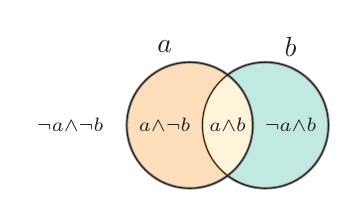
\begin{tikzpicture}
					\begin{scope}[scale=0.4]
						\begin{scope}[blend group=hard light, opacity=0.5]
							\draw[fill=color1!50!white]   ( 0:1.2) circle (2);
							\draw[fill=color3!50!white] (-180:1.2) circle (2);
						\end{scope}
						
						\draw(0:1.2) circle (2);
						\draw(-180:1.2) circle (2);
						
						\node[yshift=1cm] at (0:2) {$b$};
						\node[yshift=1cm] at (-180:2) {$a$};
						\node at (-5,0){$\scriptstyle  \lnot a \land \lnot b$};
						\node at (0,0){$\scriptstyle a \land b$};
						\node at (-180:2){$\scriptstyle a \land \lnot b$};
						\node at (0:2){$\scriptstyle  \lnot a \land b$};
					\end{scope}				
				\end{tikzpicture}
				\refstepcounter{figure}\label{fig:ven2BA}
				%	 		\caption[a]{B}
			\end{center}
		\end{minipage}\begin{minipage}{0.65\textwidth}
			\begin{equation} \left\{\;
				\begin{aligned}
					a \land b,\; a \land \lnot b,\; \lnot a \land b,\; \lnot a \land \lnot b,\; \\
					%			\smash{\overbracket{ a \land b,\; a \land \lnot b,\; \lnot a \lansd b,\; \lnot a \land \lnot b,\;}^{\text{the atoms of $B$}}} \\
					(a\land b) \lor(\lnot a \land \lnot b),\; (a\land \lnot b) \lor (\lnot a \land b),\; 0,\; 1,\;\\
					a \lor b,\; a \lor \lnot b,\;  \lnot a \lor b,\; \lnot a \lor \lnot b,\; \\
					a,\; \lnot a,\; b,\; \lnot b,\;
				\end{aligned}\;
				\right\} \label{eq:exba2} \end{equation}
		\end{minipage}
		\par\smallskip\noindent
		corresponding to the $2^{2^2} = 16$ distinct boolean expressions that can be constructed with the two primitve symbols $\{a, b\}$. The atoms of $BG$ are those elements that appear on the first line of \eqref{eq:exba2}, and correspond to the four ``atomic'' regions of the Venn diagram to their left.
	\end{example}
	
	\section{Hyper-Graphs and Information}
	We originally formalized the structure of PDGs with regular edges, which have a single source and target. However, $\IDef{}$ is most naturally understood in a setting where PDGs are modeled as hyper-graphs; we now provide an characterization in these terms.%
		\footnote{For a translation into the original formulation consult \cref{apx:hyper-vs-graph}.}
	\begin{defn}[hyper graph] \label{defn:hypergraph}
		A \emph{directed multi-hyper-graph}, (which we abbreviate \emph{hyper-graph}), is a set $\N$ of variables, and a set $\Ed = \{ \mat X \to \mat Y \}$ of hyper edges. Each edge $E \in \Ed$ has a subset of the variables $\src(E) \subseteq \N$ which we call the \emph{source} of $E$, and a second subset of variables $\tgt(E) \subseteq \N$ that we call the \emph{target} of $E$. We will often specify an edge $E$ along with its source $\mat X = \src(E)$ and target $\mat Y = \tgt(E)$ by writing $\ed E{\mat X}{\mat Y}$.
	\end{defn}
%	Although this is not always made explicit, any computation involving entropy depends on the values 
%	\begin{defn}[variable hypergraph]
%		A \emph{variable hypergraph} is a tuple $(\N, \Ed, \V)$ where $(\N, \Ed)$ is a (directed multi-)hyper graph, whose vertices $\N$ correspond to variables with values $\V$. Concretely, $\V(N)$ is the set of possible values that a variable $N \in \N$ can take.
%	\end{defn}

	\begin{defn}[Information Deficiency] \label{defn:idef}
		If $\Gr = (\N, \Ed)$ is a variable hypergraph, and $\mu \oftype{\Delta [ \prod_{N\in\N}\V(N)]}$ is a joint probability distribution over variables $\mathcal X \supseteq \N$, then the $\Gr$-information deficiency of $\mu$ is given by
		\begin{equation}
			\IDef{\Gr}(\mu) := \bigg[~\sum_{\ed E{\mat X}{\mat Y}} \H_\mu(\mat Y\mid \mat X)\bigg] - \H_\mu(\N).
% same but with src/tg instead of arrow notation
%			\IDef{\Gr}(\mu) := \bigg[~\sum_{\ed E{\mat X}{\mat Y}} \H_\mu(\mat{tgt} E\mid \mat{src} E)\bigg] - \H_\mu(\N).
			\label{eq:idef}
		\end{equation}
%		where $\H(\mat Y \mid \mat X)$ is the conditional entropy of $\mat Y$ given $\mat X$ with respect to $\mu$
%		(see \cref{apx:info} for more details)
%		, and $\H_\mu(\N)$, often written simply $\H(\mu)$, is the total entropy of $\mu$ across all variables.
	\end{defn}
	
	% Define the signed measure.
	
	\section{The Information Profile: Information as a Signed Measure.}
	
	

	


	\subsection{Constructing the Information Profile of a Distribution}
		
%	Some authors simply define $\H(Y \mid X)$ to be a difference of joint entropies $\H(X,Y) - \H(X)$. Similarly, we can write the mutual information as an alternating sum of joint entropies.
%	\begin{align*}
%		\I(X \land Y) &:= \H(X,Y) - \H(Y \mid X) - \H(X \mid Y)  & \text{[the Venn diagram without the sides]}\\
%			&=  \H(X,Y) - \H(X,Y) + \H(X) - \H(X,Y) + \H(Y)  &\text{[expanding conditional entropy]}\\
%			&= - \H(X,Y) + \H(X) + \H(Y)
%	\end{align*}
	Most quantities in information theory can be written as a difference of entropies.
	For instance, some authors simply define $\H(Y \mid X)$ to be $\H(X,Y) - \H(X)$.
	We now write the formulas for information shared between 1, 2, and 3 variables in a more suggestive form.
	\begin{align*}
		\textit{Information in $X_1$:}  && \I(X_1 &) = \H(X_1) ;\\
		\textit{Mutual Information between $X_1, X_2$:} && \I(X_1 &\land X_2) = \H(X_1) + \H(X_2)  \\
			 &&&\qquad - \H(X_1, X_2); \\
		 \textit{Interaction Information of $X_1, X_2, X_3$:}&&\I(X_1 \land &X_2 \land X_3) = \H(X_1) + \H(X_2) + \H(X_3) \\
			&&&\qquad - \H(X_1, X_2) - \H(X_2, X_3) - \H(X_1, X_3) \\
			&&&\qquad  + \H(X_1, X_2, X_3)  .\\
	\end{align*}
	This suggests that we can extend to arbitrary elements of the Boolean algebra by use of an inclusion-exclusion formula. For terms involving 3 and higher conjuncts, it is common to take such a formula to be the definition. 

	More formally, let $\N$ be a set of variables, $B[\N]$ be the free Boolean algebra generated by $\N$, and $\mu$ be a joint distribution over $\V(\N)$. As we extend entropy to these new elements, we will change the symbol $\H$ to $\I$, for compatibility with the standard notation, such as the mutual information. The information of a joint variable $\I_\mu(X \lor Y)$ which we have written so far as $\H_\mu(\{X,Y\})$ or simply $\H(X,Y)$, already tells us how to measure the entropy of joins of random variables. We simply convert meets to joins using the inclusion-exclusion rule, so that
	\begin{equation}\label{eq:inclexcl}
		\I_\mu\Big(\bigwedge_{X \in S} X\Big) =  \sum_{T \subseteq S} (-1)^{|T|+1} \I_\mu\Big( \bigvee_{X \in T} X \Big) ~,
	\end{equation}
	% (and the footsteps of \cite{JakulinBratko,BellCoInformation,})
	by analogy to the
	\href{https://en.wikipedia.org/wiki/Inclusion%E2%80%93exclusion_principle}
 		{the inclusion-exclusion rule} for probability and counting measures \cite[eq 2.7]{halpern2017reasoning}.
	
	One might worry because an element $b \in B[\N]$ of the free Boolean algebra can be represented in more than one way.
	
	\begin{inactive}
		In the formal definition that follows, we will first convert every $b$ to its canonical CNF for definiteness, but  afterwards we will show that the normalization is unnecessary, and that \eqref{eq:inclexcl} holds independent of the representation. 
	
		\begin{fact}
			For every set $S$ and $b \in B[S]$, there exists a unique finite matrix $S = (s_{i,j})$ where each $s_{i,j}$ is a literal equal either $s$ or $\lnot s$, such that 
			$\displaystyle b = \bigwedge_{i} \bigvee_{j} s_{i,j} $
		\end{fact}
		\begin{defn}
			The information $\I_\mu$ with respect to a distribution $\mu$ and a set $\N$ of variables, of an element $b \in B[\N]$, 
			\[			\I_\mu\Big(\bigwedge_{X_x \in S} X_s\Big) =  \sum_{T \subseteq S} (-1)^{|T|+1} \H\Big( T \Big) ~. \]
			%		\begin{itemize}[itemsep=0pt, parsep=1pt]
			%			\item If $\varphi = \bigvee_i X_i$, we define $\I^\N_\mu(\varphi) := \H_\mu(X_1, \ldots, X_n)$.
			%			\item For $\varphi = \bigwedge_i X_i$, we define $\I^\N_\mu(\varphi)
			%				 := \sum_{T \subseteq S} (-1)^{|T|+1} \H\Big(\bigvee_{X \in X} T\Big)$.
			%		\end{itemize}
		\end{defn}
	\end{inactive}


\begin{defn}
	We define the \emph{information} $\I_\mu^\N$ with respect to a distribution $\mu$ and a set $\N$ of variables, of a formula $\varphi \in \lang{prop}$, we inductively define
%	\[			\I_\mu\Big(\bigwedge_{X_x \in S} X_s\Big) =  \sum_{T \subseteq S} (-1)^{|T|+1} \H\Big( T \Big) ~. \]
			\begin{itemize}[itemsep=0pt, parsep=1pt]
				\item For $\varphi = \phi \lor \psi$, we define $\I^\N_\mu(\varphi) := \H_\mu(X_1, \ldots, X_n)$.
				\item For $\varphi = \bigwedge_i X_i$, we define $\I^\N_\mu(\varphi)
					 := \sum_{T \subseteq S} (-1)^{|T|+1} \H\Big(\bigvee_{X \in X} T\Big)$.
			\end{itemize}
\end{defn}
	
	\begin{defn}
		The information $\I_\mu$ with respect to a distribution $\mu$ and a set $\N$ of variables, of an element $b \in B[\N]$, 
	\[			\I_\mu\Big(\bigwedge_{X_x \in S} X_s\Big) =  \sum_{T \subseteq S} (-1)^{|T|+1} \H\Big( T \Big) ~. \]
%		\begin{itemize}[itemsep=0pt, parsep=1pt]
%			\item If $\varphi = \bigvee_i X_i$, we define $\I^\N_\mu(\varphi) := \H_\mu(X_1, \ldots, X_n)$.
%			\item For $\varphi = \bigwedge_i X_i$, we define $\I^\N_\mu(\varphi)
%				 := \sum_{T \subseteq S} (-1)^{|T|+1} \H\Big(\bigvee_{X \in X} T\Big)$.
%		\end{itemize}
	\end{defn}

	\begin{prop}
		$\I_\mu^\N$ is well-defined.
	\end{prop}

	\begin{defn}
		The \emph{information profile} of $\mu$ with respect to $\N$, denoted $\mat I_\mu^\N$, is a ($2^{|\N|} -1$) dimensional vector 
	\end{defn}

	\begin{example}
		content
	\end{example}
	

		
	\begin{prop}
		There is a factorization of $\Omega = X_1 \times X_2 \times \ldots \times X_n$ 
	\end{prop}

	This formula is given in \cite{}.

%	and the $\mu$-entropy, $\H_\mu$, can be seen as a measure over the variables $\N$, in which every $S \subseteq \N$ is measurable.
	

	

	\section{Information Quantities are Inner Products with $\mat I_\mu$}
	\section{Illustrations and Examples of $\IDef{}$}.
	
	%	\subsection{}
	%	Once again, let $\N$ be a set of variables, and $\mu$ be a joint distribution over $\N$. 
	%	The general idea is that for variables $X, Y, Z \in \N$
	
	\begin{example}
		Let $\mu$ be a distribution over the three variables $\N = \{X,Y, Z\}$. 
		%		\lipsum[1-4]
		\begin{center}%{R}{3cm}
			%			\let\varnames{X,Y,Z}
			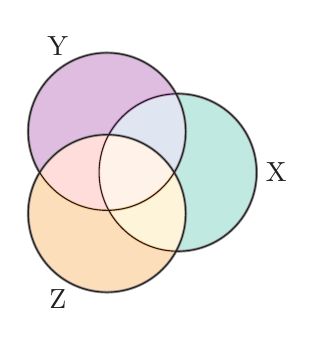
\begin{tikzpicture}
				\begin{scope}[scale=0.5]
					\begin{scope}[blend group=hard light, opacity=0.5]
						\draw[fill=color1!50!white]   ( 0:1.2) circle (2);
						\draw[fill=color2!50!white] (120:1.2) circle (2);
						\draw[fill=color3!50!white] (-120:1.2) circle (2);
%						\draw[fill=red!50!white]   ( 0:1.2) circle (2);
%						\draw[fill=green!50!white] (120:1.2) circle (2);
%						\draw[fill=blue!50!white] (-120:1.2) circle (2);
					\end{scope}
					
					\draw(0:1.2) circle (2);
					\draw(120:1.2) circle (2);
					\draw(-120:1.2) circle (2);
					
					\node at (0:3.7) {X};
					\node at (120:3.7) {Y};
					\node at (-120:3.7) {Z};
				\end{scope}				
			\end{tikzpicture}
		\end{center}
		%		\lipsum[1-6]
	\end{example}
	
	\section{Paying for structure: a symmetric extension of $\IDef{}$}
	
	% Show that it's a special case	
	\subsection*{Distributions are a specific kind of PDG}
	Let $\N$ be a set of variables whose values are given by $\V$. When we use the characterization of PDGs based on directed hyper-graphs, a joint distribution $\mu \in \Delta[\V(\N)]$ is naturally identified with a particular unweighted PDG. Specifically, the data of $\mu$ is given by the PDG $(\N, \{ E_0 \}, \V, \mat p)$ containing a single hyper-edge $E_0$ whose source is empty and whose target is all of $\N$, associated with the cpd $\bp[E](\mat x) := \mu(\mat x)$. 
	
	\begin{example}
		For a 3-variable
	\end{example}
	
	We claim that $\IDef{\N,\Ed}(\mu)$. 
	\newpage
	\appendix
	\section{Information Theory} \label{apx:info}
	\begin{defn}
		The \emph{mutual}
	\end{defn}
	\section{Correspondence with PDGs} \label{apx:hyper-vs-graph}
	\begin{defn}
		A \emph{PDH} is a PDG 
	\end{defn}
	
	% If $S \subseteq \N$ is a set of variables, we write $\H_{\mu}(S)$ to refer to the joint entropy of the variables of $S$, which is equal to $H(\mu|_S)$.
	% Let $\H_\mu(G)$ be the
	
	
	\bibliographystyle{alpha}
	\bibliography{../papers/repr/joe.bib,../db.bib,../papers/uncertainty.bib}
\end{document}
